\documentclass[a4paper,12pt]{article}
\usepackage{fontspec,xunicode,xltxtra}
\usepackage{booktabs}
\usepackage{indentfirst}
\usepackage{graphicx} 
\usepackage[SlantFont]{xeCJK}

\setCJKfamilyfont{mincho}{TakaoExMincho}
\setCJKfamilyfont{gothic}{TakaoExGothic}
\newcommand\ja[1]{{\CJKfamily{gothic}#1}}
\setCJKmainfont[BoldFont=WenQuanYi Micro Hei]{Adobe Song Std}
\setCJKsansfont{WenQuanYi Micro Hei}

\setmainfont[Mapping=tex-text]{Liberation Serif}
\setsansfont{Liberation Sans Narrow}
\setmonofont{Liberation Mono}
\XeTeXlinebreaklocale "zh"
\XeTeXlinebreakskip = 0pt plus 1pt minus 0.1pt

\linespread{1.3}
\usepackage[top=25mm,bottom=20mm,left=30mm,right=30mm]{geometry}

\renewcommand{\contentsname}{目录}


\author{yx-wh}
\title{Matz}
\begin{document}

\newpage
松本行弘的黑客生活
\setcounter{tocdepth}{2}
\tableofcontents
\newpage

\section{第1回 与黑客相遇}
究竟什么是Hacker呢? 松本行弘的人气连载——介绍了黑客不为人所知的生态和心理——在ITmedia登场!「黑客的生活方式或许能让你成为更好的程序员——不过我也打不了包票。」

大家好,我是松本行弘。在世间以Ruby编程语言的作者这一名字为人所知,职业为程序员,自称黑客。这次连载我希望能介绍介绍我们这些「黑客」的生态和心理。

\subsection{什么是「黑客」?}

「黑客」指的并不是通过网络入侵他人系统、破解密码的坏家伙——话说,最近很少听到这种错误的用法了呢。

Hacker这个词正如其字面意思所示,指的是「实践hack之道的人」。Hack的本义是「用斧头(之类的)猛砍」的意思,后来意义演变为「搞定了程序」。「搞定」也许会给以一种应付差事的感觉,但其实它的言外之意是说工作完成得快,与好坏无关;优秀的工作可以称之为“hack”,为了应付死线(deadline)纯粹交差的工作也是“hack”。热爱上述工作的黑客,就是那种一坐到电脑前(或者任何可编程的东西前)就沉迷得不想再起来的人。

在黑客们自己编纂的用语辞典《jargon file》中,对黑客有如下定义。很长吧?仅由此便可知黑客们对于“hacker”这个词有着多么执着。
\begin{quote}
	\begin{itemize}
		\item 一个热衷于探索可编程系统的细节以及如何扩展它们的功能的人,他/她/它与绝大多数用户不同,后者只想学会他们工作中所需要的最低限度的东西。
		\item 热衷于(甚至像是鬼上了身似的)编程本身,而不是把编程弄成一套理论的人。
		\item 能够接受黑客价值(hack value)的人。
		\item 一个擅长很快写出程序的人。
		\item 某个特定程序的专家,以及经常使用它进行工作的人。例:“UNIX Hacker”。
		\item 任何领域的专家或狂热的爱好者。例:“天文Hacker”。
		\item 热衷于「用创造性克服或回避极限」这样一种智力游戏的人。
		\item (误用)四处游荡、探索机密信息的恶意干涉者。比如口令Hacker、网络Hacker。正确的表达是craker。
	\end{itemize}
\end{quote}
在其他人看来,黑客是化「看似不可能」为「可能」的人。在对编程缺乏了解或是知之甚少的人看来,黑客就像是魔法师。在「沉浸于自己喜欢的事物」这一点上,黑客是幸福的;但黑客中有不少,都和「财富」「资产」这样的词绝缘。但是,世上也有黑客属于例外,他们发现了把自己的才能变为财富的方法。

\subsection{好黑客·坏黑客}
做侵入系统那样坏事的人之所以被称之为黑客,是因为那样的事也曾是「有创造性的智力挑战」,因而有黑客去做。
和一般人相比,绝大多数黑客的伦理观都显得有些轻微的错位。「有时候,比起遵守法律做个良民,满足知性的好奇心显得更为重要」这种心情,不是不能理解。但是,一个人是不是黑客和他/她/它是不是坏人是完全无关的。倒不如说,如果有真正的黑客侵入了系统,那他/她/它的动机恐怕也是「想试试看」「我想证明自己做的到」而不是「从中获取经济利益」这种不正当的动机。黑客中有许多人对于金钱之类的物质追求其实不怎么在乎。

\subsection{你是黑客吗?}
那么,各位读者,你是黑客吗?既然都点到这个网站上来了(抱歉了,ITmedia),你肯定是喜欢计算机,对编程也有兴趣吧?此外,如果你不满足于只做一个「普通的电脑用户」(那样的人肯定读的是教如何使用Windows的杂志),而是使用具备黑客特质的类UNIX操作系统的话,那么你是黑客的可能性可以说是十分的高啦。

根据我的假说,是否拥有黑客特质,取决于是否满足以下两个条件:

首先是「你有创造欲吗?」这个问题。具有狂热特质的人大体趋于分为两类,「收藏爱好者」和「创造爱好者」。当然,也有人同时具有两种特质,这时问题就取决于在编程上你的哪种特质显现得更多。收藏爱好者关心机器的配置和新旧、以及计算机和软件的使用方法,但创造爱好者则是像「没有的话我自己造」「这里不给力,我要改改」这样,努力的改变着「世界」。所以,他们喜欢的是能够按自己的喜好进行个性化的软件,特别是有可编程性的软件。对于做东西的热情,这难道不是黑客特质的第一要素吗?

其次是「你是否做事『不住车』?」。这个说法有点奇怪,不过我所知道的黑客,几乎都在某方面「刹不住车」。普通人遇到了一个觉得难以解决的问题想放弃的时候,黑客却会想再接着试试。黑客继续做下去的理由,有时是无知,有时是无谋、自信过剩,也有时是拥有超出常人的能力;但总之他们比常人更不愿放弃。所以他们才能成他人所不能成之事——当然也有时候会失败就是了。不过,黑客预备役们也都是重复着不为人知的失败才成长为黑客的。

\subsection{黑客的三大美德}
如今无人不知的脚本语言——Perl的作者,Larry Wall是当代一流的黑客。他说,程序员有三大美德:懒惰、傲慢、缺乏耐性\footnote{Larry Wall对三大美德的定义

\begin{itemize}
\item 懒惰(laziness)\\ 
驱使你极力努力以减少精力的总的消耗的美德。为了节省劳力而开发的程序在被他人所使用后,为了不至于一一回答他人在使用程序时的问题而开始编写文档。因此,懒惰是程序员最重要的美德。此外也正是由于这一点,才有了本书(《Programming Perl》)的存在。

\item 缺乏耐性(impatience)\\ 
发现计算机没干事情时候的愤怒。这成为编写不仅能够对你的指令进行回应、而且还能预测实际的指令(至少看上去是如此)的程序的原动力。因此,这是对于程序员第二重要的美德。

\item 傲慢(Hubris)\\ 
如同碰到了宙斯的怒火一般(?),自尊心很高。这是编写(和维护)不为他人所批评的程序的原动力。因此,这是对于程序员第三重要的美德。
(《Programming Perl》,O'reilly Japan)
\end{itemize}
}。当然啦,这里的「程序猿」指的是具备黑客特质的人。
可是,「懒惰」也好,「傲慢」也好,「缺乏耐性」也好,这些怎么看都像是描述缺点的词汇怎么成了「美德」了呢?Larry自己则是给这些词下了如下的定义。「为了让事情变得轻松一点而不辞辛苦」,这话听上去奇怪;不过虽然黑客对于无法满足自己求知欲的事情,连一根指头也不想动,但对于自己想做的事情,往往再多的辛劳也不以为意。此外,由于傲慢和缺乏耐性的缘故,黑客讨厌被计算机牵着走。对于生成导入计算机的数据这样的重复机械作业,他们会编写脚本,把机械作业留给计算机,或者开始开发能够一劳永逸解决此类作业的工具。在一般人看来,这也许是本末倒置的行为。但是,黑客就是这样的人。

我想在这个连载中考察这样的黑客们的生态和心理。黑客的生活方式或许能让你成为更好的程序员——不过我也打不了包票。

\rightline{本文由开源杂志2005年4月号的《松本行弘的黑客生活》重构而成。}

\section{第2回 对键盘的讲究}

\subsection{键盘和马鞍}

注重提高生产力的手艺人对自己所用的工具是很挑剔的。对于当代的「IT手艺人」来说,最常接触的工具,难道不是键盘吗?这个月我们就来研究研究黑客对键盘有什么讲究。

在黑客键盘中最有名的,恐怕是Happy Hacking Keyboard吧。HHKB是由东京大学的和田英一名誉教授\footnote{和田英一名誉教授

和田教授以参变管(Parametron)计算机的开发、Algol N的设计、和田研字体的开发等为人所知。}(他可以说是国内黑客的「先驱」)所策划、监修的商品,被赞誉为「为黑客而生的键盘」。其特点有:讲究的键轴、与Sun Type3 Keyboard\footnote{Sun Type3 Keyboard

非常有名,我在学生时代也非常喜欢使用。我还记得,之后SPARC Station附带的Type4键盘由于品质过于低劣,让我很失望。}兼容的键位布局、最低限度的按键数目\footnote{最低限度的按键数目

早期的HHKB上连方向键都没有。需要使用方向键的时候使用Fn+字母键代替。由于很多人抱怨实在是难用,Happy Hacking Keyboard Lite之后增加了小方向键。}以及因此所致的空间节省。和田教授对键盘的讲究,从下面的这个对话中可见一斑:

美国西部的牛仔们,在马死了之后就把马留在原地。可不管在沙漠里走多久,背着的鞍也决不会丢下。这是因为,马只是消耗品,鞍却是和自己磨合好了的「人马接口」。放到现在就是说,PC不过是消耗品,键盘才是陪伴你一生的重要的人机接口。这一点可不能忘。

最近\footnote{Matz这里说的是2005年}的电脑,只要几年性能就落伍了。CPU变慢(其实变慢的不是CPU而是软件吧?)、硬盘容量不够,所以总是得换新的。可是,在买了新的主机时,用称手的高档键盘却可以一直不换。可以说,正因为键盘是每天要接触的人机接口,才需要这么讲究吧。

\subsection{十人十色}

黑客对键盘的讲究有许多不同的表现形式。我认识的一个Perl Hacker,西文输入使用的是德沃夏克键盘(Dvorak Keyboard)\footnote{德沃夏克键盘(Dvorak Keyboard)

August Dvorak博士开发的键盘按键排列。也称作Dvorak Simplified Keyboard(DSK)。与之相对,普通的键盘排列则称作QWERTY排列。Dvorak键盘排列如图1所示,元音字母集中在左手,因而易学易打。

%   '  ,  .  p  y  f  g  c  r  l  / = 
%    a  o  e  u  i  d  h  t  n  s  - 
%     ;  q  j  k  x  b  m  w  v  z 
%
%   "  <  >  P  Y  F  G  C  R  L  ?  +  
%    A  O  E  U  I  D  H  T  N  S  \_ 
%     :  Q  J  K  X  B  M  W  V  Z 
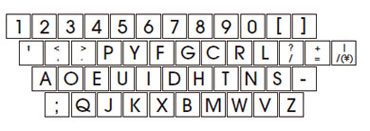
\includegraphics[scale=0.5]{hlfig1.jpg}

图1 Dvorak键盘排列
},日文输入则使用T-Code\footnote{T-Code

无联想2键日文输入方式。将码长为2的编码分别指派给不同的汉字、平假名、片假名,直接输入。由于不用选字,输入速度很快,但弱点在于没记住编码的汉字就打不出来。不过,只要记得平假名,就可通过平假名选字变换成汉字(译者:类似于五笔输入法中加入了拼音),这时系统会告诉你这个字的编码。}。讲究键盘和按键排列的人我认识不少,但同时使用Dvorak和T-Code的,我只知道他这一个。

产业综合研究所的增井俊之也以黑客而闻名,他似乎就把键盘的按键排列给改了。《Rubyist Magazine》\footnote{《Rubyist Magazine》

「日本Ruby会」的有志者发行的Web杂志。其中名叫Rubyist Hotlinks的连载上刊登有和Ruby相关的著名人士的采访。}第5期中的采访提到,他把最近较少使用的分号键给换成了回车。
\begin{quote}
增井:自那以后,最近就注意到,我很少使用分号键呢。键盘打字的时候,小指不是正好在分号上嘛。这是个不错的键位,而且在C和Perl之类的语言中经常用到,但是Ruby中不用呢。可是不用的按键居然在这么好的位置上,是在是可惜啊,于是就把它换成了回车键。

众人:(爆笑)

增井:所以我现在的机器,右手小指的按键都改成回车啦。这样的话手都不用怎么动了呢。普通人的话,敲退格要动右手,敲回车也要用右手,手有很多无效的动作呢。输入日文的时候恐怕也会有很多手的动作。可是,把那个键设成回车之后,手几乎不用移动就能轻松输入了哦。
\end{quote}
为了配合Ruby专门改变按键排列,正是「刹不住车」的黑客式的态度呢。在这个采访中,还有其他许多得以窥见增井的黑客人格的基准点的段落\footnote{窥见基准点的段落

我印象最深的是,把集成电路芯片串起来做成微机的故事。1970年代后半正是Microcomputer Kit(小)火了一阵的时候,他看之后就觉得,「那些买Kit的人『实在是弱爆了,电路啥的别人都搭好了,有什么意思』。自己想电路、买齐芯片、布线、所有的控制程序都是自己写,那才叫自制的电脑好吧。」——看来此人真是非同寻常啊。},大家也一定不要错过。

\subsection[日文输入的键盘排列——「kyuri改」]{日文输入的键盘排列——「kyuri改」\footnote{译者:现在不会日语,将来也不想学日语的同学,可以跳过了。另外我受到汉语双拼的启发,也搞了自己的日文键盘排列。}}
%标题直接插入脚注会悲剧

好吧,再说说我自己的事情。我属于笔记本党,所以没法像和田教授那样搞「使用终生的键盘」了。

即便如此,对于按键排列我还是有讲究的。首先是西文输入中,日语键盘(所谓的JIS排列)我也按照英语键盘(所谓的ASCII排列)来用。这是因为ASDF这一行中「Enter」旁边的按键的数目实在让人在意。在美式键盘中,这里是没有按键的,所以「`」在不同的美式键盘中会排列在各种不同的地方\footnote{「`」在不同的美式键盘中会排列在各种不同的地方
	
美式键盘中,有的「`」键在1的左侧,有的在键盘右下方,各有不同。这不科学!},实在让我不喜欢。此外,对于JIS排列中「[」和「]」不是横着排列在一起而是分两行排列,我也感到不满——明明「(」和「)」是横着排在一起的说。我之所以喜欢ASCII排列,我最早上班的单位所使用的SONY的工作站(NEWS)的键盘就是这种「虽然是ASCII排列但Enter的左边多了个键」的,或许是其原因之一。

对按键排列,其实我还有一个讲究,就是日文输入使用了我独自定义的按键排列。我称之为「kyuri改」。

「kyuri改」是一种左手辅音右手元音的按键排列。例如,先按「G」(其实是西文输入时的Q)再按「U」(西文输入时的J)就能输入「\ja{ぐ}」(日语平假名gu)。基本上是左手和右手交替运动,所以可以很有节奏的输入文字。

%   G  M  N  R  P  V  ゃ ゅ ょ ー    
%    Y  H  K  S  T  A  U  I  O  E  
%     Z  W  B  D  小 ん っ 、 。  
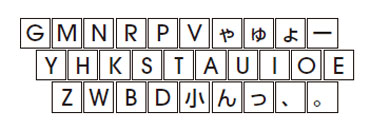
\includegraphics[scale=0.5]{hlfig2.jpg}

图2 「kyuri改」

像「\ja{きゃ}」这样包含拗音的文字,怎是在辅音后按「\ja{ゃ}」这个专用的拗音键。除此之外的小假名都使用「小」键输入:

「H」「小」「A」→「\ja{ふぁ}」

罗马字输入方式中容易输错的「\ja{ん}」和「\ja{っ}」都分配了单独的按键,所以再也不用担心「\ja{な行}」和「\ja{ん}」相混淆,或者以「\ja{っ}」结尾的句子难打啦。

使用Canna这种日文输入法的读者,可以使用我所用的kpdef文件来尝试「kyuri改」的效果。下载地址\footnote{译者:已成死链}

使用Canna附带的mkromdic从kyuri.kpdef生成罗马字假名转换表(文件名是以.开头的)吧。之后,把转换表放到家目录里面,再在.canna文件里面加上

(setq romkana-table "转换表名称")

这一行,就可以使用kyuri改啦。

「kyuri改」并非是我完全原创的想法,而是之前受到狩野弘树1991年编制的「kyuri」\footnote{kyuri

原版kyuri的信息可以参照狩野的网站。}这一排列的启发才诞生的。大概是1992年左右的时候吧,那时的我对自定义键盘排列非常感兴趣,所以深深地沉迷于「在日文输入中使用『kyuri』」这个想法而不能自拔。不过实际使用后还是觉得有些地方不太好用,于是按自己的指法习惯,移动了难打的按键的位置,并使得连续地按拗音键可以输入「\ja{ゃあ}」「\ja{ゅう}」「\ja{ょう}」等等。做了这些改进之后,诞生的就是「kyuri改」。

像这样对称手工具的追求,乃是黑客特质之一。各位读者,试着将自己身边的工具用到称手的极致吧。或许这样就能体会到黑客的心情了。

\rightline{本文由开源杂志2005年5月号的《松本行弘的黑客生活》重构而成。}

\section{第3回 黑客与工作}

具有黑客倾向的人们,说实在的,不太适合商业活动。可是,不管是多么牛的黑客,也不能靠西北风过活啊。所以这回我们来说说黑客的工作生活吧。

具有黑客倾向的人们,说实在的,不太适合商业活动。毕竟,他们可是以「懒惰」「傲慢」「缺乏耐性」为美德的人,沉迷于自己喜欢的事情,但对于自己讨厌的事情就难以忍受。可是,做生意可不是这么轻松的事情。

黑客也是人。困了要睡觉,饿了要吃饭。不管是多么牛的黑客,也不能靠西北风过活啊。所以这回我们来说说黑客的工作生活吧。由于是从我身边的极少数样本那里所获取的信息,充满了独断和偏见,各位读者一定要预先了解这一点。

\subsection{论文和毕业最要命}

见到黑客最多的地方,果然还是大学和研究所。以UNIX和C(AT\&T贝尔实验室)、BSD(加州大学伯克利分校)、TeX(斯坦福大学)为首的许多黑客技术,都是从大学和研究所产生的。可以毫不客气地说,这半个世纪的计算机科学都是由从事研究工作的黑客所发展的。

这些领域是既能满足黑客的求知欲、又能作为职业满足个人生活的重要领域。看上去对于黑客来说应该是理想的工作了吧,可是人世间是没有那么轻松的事的。在研究员组成的小社会中,业绩使用发论文的情况来评价的。对于只爱写程序不爱干其他事情的软件黑客来说,要他写论文简直是要了他的命。考虑到最大化对人类整体的贡献的话,「擅长写程序的黑客光写程序」或许是更好的选择,可惜的是社会的构造并不允许他们这么做啊。

除了大学的教职工,学生黑客也是如此。学生们充满着朝气和与之相应的行动力(当然也有学生并非如此),而且绝大多数都有着充裕的时间\footnote{译者:本科化学狗悲惨地飘过,表示化学和生物都是苦B},所以有的能够做出非常有趣的作品。最有名的学生作品,恐怕是Linus Torvalds在他赫尔辛基大学时代创作的Linux。学生黑客既有考试和打工等等障碍,又有「终究会毕业」这一严峻(?)的现实。Ruby界也有这样的例子,我印象最深刻的,有以Intel x86系统为对象的JIT编译器rubyjit和同一作者的将ruby转换为c的rb2c。两个都是很有趣的工作,但是伴随作者的毕业都停止了开发,而愿意接盘的勇者却没有出现……非常遗憾。

\subsection{本末倒置}

学生毕业之后就要找工作了。刚才我们已经讨论了留在大学当研究院的案例,现在再来看看在企业就职的情况。虽说人数不多,但是也有人是在工作后参与软件开发业务中发现开发程序的乐趣进而觉醒了黑客之魂的。

已经参加工作的黑客的多数属于「副业型」。一边将自己的本职工作作为业务上的需求而完成,一边将真正有趣的编程活动作为自己的兴趣而进行。工作中的忙里悠闲啊,下班后在自己家里鼓捣啊,削减睡眠时间啊,诸如此类。这个嘛,只要是有自己感兴趣的事情(即使不是编程)的人,对于上述现象也是感同身受吧。为了吃饭而多少干一些活,为了自己的兴趣而写程序。或许这是很稳定的生活方式呢。

问题在于黑客的人格。由于黑客往往具有「刹不住车」的倾向,总会渐渐地钻到自己喜欢的方向里面去。此外,将成果作为开源软件公开之后,随着软件用户数量的增长,支持和维护工作所花的时间也会变成一个不小的数字。我最初也是在上班当程序员时,在工作之余开发了Ruby。几年间一直在工作中抽出时间开发Ruby,但随着Ruby使用者的增加,邮件列表上的邮件到了一天几十封的程度,这时仅仅是读邮件、写回覆、修正别人报告的bug,也要耗上大半天。到了这时,原来的做法已经不可持续了。这时,副业型的黑客就到了不得不选择接下来的行动的时候。

\subsection{接下来的一招}

可以考虑的选择有好几个。首先想到的是以下几个吧。不论那个都是实际可行的。
\begin{itemize}
	\item 成为程序员中的自由职业者。把工作的期间和Hack的期间明确地分开。
	\item 说服上司理解黑客
	\item 跳槽到理解黑客的单位
	\item 自己创业
\end{itemize}

成为自由职业者有着工作缺乏稳定这一难处,但可以做自己想做的工作。但是,要能自己找到工作,关系是不可少的,对自我管理能力也有要求。黑客里面似乎自我管理能力弱的人很多的样子啊……

至于说服上司,WideStudio的平林是个例子。他应征了IPA\footnote{IPA

信息处理推进机构(日:「\ja{情報処理推進機構}」)。经济产业省主管的独立行政法人。除了举行信息处理技术员考试和进行各种支援工作,兼有运营提供安全信息的JP-CERT。}的「未踏Project」\footnote{未踏Project
	
正式名称是「创造前所未有的软件的事业」(日:「\ja{未踏ソフトウェア創造事業}」)。这个工程以发掘「开发前所未有的软件的个人」为重点。我曾在2000年度(第1届)获得采纳。},通过被认定为「超级创造者」\footnote{超级创造者

「未踏Project」中取得了令人惊艳的成果的人,由IPA所授予的称号。不是所有人都能获得的——我就没有。}获得了上司的理解,成功地将自己hack的结果作为工作得到了认可。像这样利用「未踏Project」使自己的hack获得世人承认的例子还有很多。

我自己则是在跳槽后找到了自己的安乐窝。我1997年跳到了我现在工作的地方——网络应用通信研究所,转职当时是作为「Ruby开发者」被采用的。这家公司对于如何使用黑客颇有心得,给我提供了很舒服的职场环境。托了公司的福,跳槽后的这八年来,能一直舒适地完成工作。绝大多数黑客其实很少有发大财的野心,只要有吃喝不愁的收入、适当有趣的工作和技术挑战、以及和其他黑客的良好交流就很满足啦。由于黑客的生产率相当于普通技术人员的数倍~数十倍,对于公司来说是太赚啦。此外,著名的黑客还有作为企业的看板或者广告牌的作用,这方面也是公司能够有效活用的。

但即便是黑客也是有许多种不同类型的人的,其中也有些有野心的类型。感觉大概就是,比起hack程序,更喜欢利用技术去hack社会吧。在风投文化发达的美国,也能看到若干将黑客创造出的技术作为卖点的风投企业。因此成功而成为大富翁的黑客也是有的。例如,将Lisp作为「秘密武器」成功做成了Viaweb这个网购平台提供服务的Paul Graham(或许作为《黑客与画家》\footnote{《黑客与画家》

中文版由阮一峰译,人民邮电出版社出版。}的作者更有名)、以Netscape Naviagtor的Lead programmer闻名的Mark Andreessen等。在创业和风投不太流行的日本,没有著名的「创业黑客」\footnote{没有著名的「创业黑客」

原On The Edge(现livedoor)CTO的小饲弹或许是例外的日本创业黑客。或许是因为他的品味很不日本的缘故吧。};但是考虑到日本的将来、社会的变化,我想,最好能出现更多像这样的黑客。

\subsection{双赢关系}

光强调黑客坏的侧面,那么黑客就会变为缺乏社会整合性的普通懒惰职员。不过,黑客们不仅是有着很高生产率的程序员,也是对新技术反应敏感的触觉的拥有者。这样的人才,如果能够灵活运用,难道不会成为企业的「秘密武器」吗?只要把黑客放到满足他们求知好奇心的工程中,放到舒适的环境里他们就很happy了,而企业也因为运用先进生产力提升了业绩而happy;这样的场面要是能普遍出现,那样就更好啦。

\rightline{本文由开源杂志2005年6月号的《松本行弘的黑客生活》重构而成。}

\section{第4回 Emacs对Vi}

即使是黑客,也不是千人一面。黑客中也存在着各种兴趣、各种文化。而且他们往往因自己的意见和文化而产生争论。这回我就以「Emacs还是Vi」为例来眺望一下黑客文化圈吧。

\subsection{争论的neta}

即使是黑客,也不是千人一面。黑客也有各种各样的。把那些只做坏事的「自称黑客」除开不算,黑客中也存在着各种兴趣、各种文化。而且他们往往因自己的意见和文化而产生争论。像这样的争论主题有很多典型的有:「哪个编程语言最优秀啊?」「哪个操作系统最好啊?」「最厉害的编辑器究竟是Emacs还是Vi啊?」等。这回我就以最后问的那个「Emacs还是Vi」为例来眺望一下黑客文化圈吧。

\subsection{从TECO进化而来的Emacs}

最早的Emacs,是理查德·斯托曼(Richard Stallman)为TECO编辑器开发的宏。Richard Stallman以GNU的运动而闻名,但其实他本来也是超一流的黑客,写起代码也是不含糊的,这一点可别忘了。TECO是具备宏功能的行编辑器(Line Editor)。Stallman则使用它的宏功能,编写了最早的Emacs——和TECO不同,Emacs是全屏幕编辑器。

据记载,在TECO上实现Emacs是1976年的事情。后来,Java的设计者詹姆斯·高斯林(James Gosling)在1981年开发了UNIX版的Emacs。Gosling开发的Emacs(通称Gosling Emacs或Gosmacs)拥有一种叫做MockLisp的、类似Lisp的语言来扩展它的功能。但是Gosling把Gosmacs的著作权卖给了UniPress公司,Stallman不能以Gosmacs为基础来开发新的Emacs。

结果,不能以UniPress Emacs为基础进行开发的Stallman再次从零开始开发Emacs。这就是现在广泛使用的GNU Emacs。GNU Emacs参考了Gosmacs的扩展性,但使用的并不是MockLisp那样的山寨语言,而是内含了更为「正宗」的Lisp——Emacs Lisp。Emacs本体只包含了基本的编辑功能和Emacs Lisp,绝大多数方便的功能都是随后使用Emacs Lisp实现的。也就是说,普通用户也能用Emacs的基本功能为基础实现各种各样的功能。其实,Emacs中(包括支持编程语言的各种模式在内的)各种编辑辅助功能,都是由用户提交的代码所实现的。此外,除了文本编辑器,Emacs还提供了无所不包的扩展功能,例如阅读电子邮件、新闻组、浏览Web、玩游戏之类之类。Emacs已经不单单是一个编辑器了,它已经发展成了一种集成环境、甚至可以说是一种操作系统了。

\subsection{从ed进化而来的vi}

vi是VIsual editor之略,它是由BSD的核心人物、曾长期担任太阳微系统公司(Sun Microsystems)副总的比尔·乔伊(Bill Joy)在1976年开发的,是以UNIX的标准行编辑器ed和ex为基础,加入了全屏编辑功能的产物。它能轻松地通过ed macro进行非对话模式的作业,随时都能安心地回到行编辑的状态。到了现在,需要这两项功能的机会应该是很少了,不过我在当学生的时候,有时因为终端出了问题,在行编辑模式下使用过vi\footnote{在行模式下使用vi

当不知道全屏编辑所必需的、终端的控制字符的时候,vi会在行模式下启动。也就是说在ed兼容模式下工作啦。}。

话说我学生时代有个叫E君的朋友,他那时总爱用行编辑器ed。有天他感叹道,「要是有个编辑器既能像less那样直接看满屏,又能用ed命令编辑就好啦。做个lessed吧\footnote{做个lessed吧

那时要是没告诉他vi的存在,或许现在就有能和Emacs、vi三分天下的黑客用编辑器了呢。可惜啊!}」,于是开始弄(hack)less的源代码。我不忍卒视,就告诉他「那个就是vi啊」,他深受震动。那是1988年的事情。每天都在用UNIX却不知道vi,究竟是大牛呢,还是奇葩呢?

\subsection{新泽西PK麻省}

vi可以说是UNIX哲学的体现。在新泽西州贝尔实验室出世的UNIX,它的哲学强调「将许多单一工具组合起来的灵活性」。熟谙UNIX工具的人,肯定会想起把各种过滤器组合在一起的「管道处理」。将cat、grep、awk、sed、nroff、pic、tbl等单功能工具用管道连在一起工作,可以说是一种高超的技艺。在UNIX哲学看来,编辑器也被看作上述工具的一种。获取两个文件的不同之处的diff,指定-e选项就输出ed脚本。将输出结果的最后加上「w」交给ed,就能自动改写并保存文件。不过,这种方式的危险在于,只要文件略有更改,就会导致悲惨的结果,所以现在人们几乎都在使用略微聪明一些的patch命令,而不是ed。

如上所述,vi这个工具反映的是「Small Is Beautiful、Keep It Simple」(小既是美、保持简约)的思想。

与之相对的Emacs反映的是另一种思想。Emacs现在由于常在UNIX上使用,容易被看作UNIX系编辑器,但其实它原先不是在UNIX上开发的。

Emacs(被认为)反映的是MIT(美国麻省理工学院)的Lisp文化。Lisp于1958年诞生于MIT\footnote{Lisp于1958年诞生于MIT

Lisp之父是约翰·麦卡锡(John McCarthy)。将其作为实际的编程语言开发出来的是史帝芬·罗素(Steve Russell)。}。(Matz写作本文的时候)已经快50年了呢。几乎所有的Lisp处理系统,都是通过交互对话进行处理的;采取的开发方式则是「将程序所必须的函数一个个定义出来,逐渐完善开发环境」。可以想像,在这样的环境中成长起来的Lisp Hacker看来,「在Lisp处理系统中加上编辑功能,逐渐将其完善成编辑器」这种做法,是非常自然而然的。考虑到1970年代的Stallman是著名的Lisp Hacker,可以说是「有了他才有了这个编辑器」呢。

Emacs的魅力在于其扩展性,也可以叫作「可编程性」。将Emacs作为开发的基础,利用其本身具备的屏幕操作等基本功能,可以有效地开发程序。我自己就开发了许多辅助日常编辑的Emacs用小工具,还开发了支持Ruby编辑和缩进的rubymode、Emacs上的两个邮件阅读器(email和morq\footnote{morq

morq是基于全文检索的邮件阅读器。})。

但是,Emacs在作为编辑器的同时又吸纳了各种功能,导致它变得越来越复杂、臃肿。有人称其为「厨房水槽」。

UNIX思想通过小工具的组合提供灵活性;Lisp思想通过可编程的工具提供灵活性。两个编辑器的对立同时也是两种思想的对立。

\subsection{NASA乱入}

不过,由于后来Emacs被看作UNIX上代表性的编辑器,战况变的有些复杂。双都被认为是UNIX的好机友,以往的UNIX对Lisp的这种容易看出的对立模式变得难以识别。随后,由于另一个「厨房水槽」Perl的参战,原先的对立模式变得完全看不出了。

Perl试图将UNIX文化中通过个别工具提供的功能全打包到一种语言当中。开发者Larry Wall(当时在NASA喷气推进实验室工作)是否受到Lisp文化的影响,并不好说;但他广为展示了「厨房水槽」方式的有效,这倒是毋庸置疑的。最终,Perl成了UNIX文化和Lisp文化之间的桥梁。

各位读者在看到「Emacs对vi」的争论时,请追寻它们身后UNIX和Lisp思想对决的轨迹吧。思想虽然不停地在改变外形,但它们一直活在黑客们的文化中。

\rightline{本文由开源杂志2005年7月号的《松本行弘的黑客生活》重构而成。}

\section{第5回 黑客环境问题}

人类虽然积极地改造了自己周围的环境,但是现在恐怕只有一部分人能够积极改造赛博空间的环境。一切东西不亲手改造过就不放心的黑客,与其说是处在进化的最前沿,倒不如说是被时代所遗弃的旧人类(Old Type)呢。

\subsection{改造环境的能力}

题目中虽然有「环境问题」这个词,但我在这里要讨论的并不是地球暖化之类的话题,而是有关黑客生活的空间——亦即计算机环境的。

地球上生活着种类多得不可胜数的生物,但要说分布范围之广,恐怕没有超过人类的。从炎热的赤道正下方到严寒的极地,都有人的踪影。但人类的繁荣不是因为人这种生物具有很好的耐力\footnote{具有很好的耐力

要说具有很好的耐力的生物,恐怕非水熊虫(缓步动物门)莫属吧。该生物身长约1mm,可以忍受的温度从-272℃(接近绝对零度)到151℃,放到真空中也没事。}是由于人类能够通过衣服和房屋控制自己周围的环境,才得以实现的。不管外边多么冷也能建造舒适住所的能力、特别是积极改造自己周围的环境的意欲,才是人类实际控制地球的理由吧。但是,战天斗地的积极过了头,反倒把环境的平衡弄得要崩溃,那麻烦就大了;不过这已经是另一个完全不同的问题了。

人类就是这样改造着环境。但是,面对随着计算机的登场而出现的赛博空间,现在能积极地改造它的,恐怕只有一少部分人。

\subsection{随处可见的计算机}

现在,在人们的身边,到处都是高性能的计算机,其数量是20多年前所无法比拟的。最近的计算机有着远远超越过去超级计算机的性能。此外,在数量上的发展也是日新月异,电视机、相机、汽车、电饭锅內都嵌入了电脑芯片。在日本这样的发达国家,几乎每个人都已经拥有了某种形式的计算机了吧?此外,基本人手一台的手机,就是兼具通话功能和网络访问功能的移动式计算机。看到在有轨电车上、在路边对着手机按来按去的人们,不得不感叹如此厉害的东西已经成了现实。人人拥有、在日常生活中频繁使用的移动式计算设备,在不久的过去还只是科幻小说中才有的未来景观。

此外,非嵌入式的通用计算机,也就是所谓的PC\footnote{所谓的PC

在日本,PersoCom(PERSOnalCOMputer)[\ja{パソコン(パーソナルコンピュータ)}]这种称呼更为世人接受。体验过「MiCom」(MIcroCOMputer,微机)[\ja{マイコン(マイクロコンピュータ)}]的那代人,对「PC」这一缩写总有些抵抗。Personal Computer[\ja{パーソナルコンピュータ}]难道不该缩略为「PERCOM」[\ja{パーコン}]么?不,「PERCOM」这个名称我也不喜欢。对于Super Computer[\ja{スーパーコンピュータ}]的缩写SuperCom[\ja{スパコン}]也觉得不适应。
【译者:日语中「微机」是个四音拍的词,它各取了「微型」和「计算机」这两个词的前两拍。个人电脑和超级计算机虽然也都是四音拍的词,但是取的却不是「个人」或者「超级」的前两个音拍。】}普及率也很高,计算机使用人口的增加远超过去。可是,绝大多数人只是把计算机用作完成特定工作的工具,有时上上网、用字处理软件写写文档、用电子表格软件做做统计什么的,但完全不它来编程。我的家人也和大多数人一样,多少用上了电脑。孩子们的学校里有了微机室,也有某了个关于信息技术的课程。也许是因此,他在我不在的时候就打开电脑的电源,上网看动画、玩游戏。

将计算机作为工具使用,将别人给予的功能原封不动地使用,这并不坏。可是,让自己适应已经给定的环境,感觉像是人类(改造环境本能)的退化。其实,在信息技术专业强的大学中,现在已经有大量虽然用过计算机但对编程一窍不通的新生入学,让人感到困惑。这不是一次两次的事情了。

\subsection{用编程定制}

在我最开始接触计算机的时候,计算机是为了编程而使用的工具。在只有BASIC的电脑上,能做的事情很有限;尽管如此,编程也是很有趣的经历。当时的计算机\footnote{当时的计算机

从70年代晚期到80年代早期,面向个人的计算机被称作「微机」。个人电脑的缩略,PC,是后来才登场的。}用户,几乎人人都能多少写些程序。那时的计算机处理能力弱,功能也少,但通过编程体验到了「让自己做自己想做的东西」的感觉。这么看来,这20多年间,计算机的存在方式也变了不少呢。

可是,不管是过去还是现在,黑客这种生物都是「懒惰」、「傲慢」、「缺乏耐性」的,所以难以忍受像是「满足于别人所给予的环境」、「为了环境而改造自己」之类的事情。黑客坐在电脑——电子计算机——面前,是无法忍耐像「按计算器」那样的操作的。他们由于傲慢,觉得造那样的事情好像让自己成了计算机的奴隶;由于懒惰,难以忍受单纯重复作业;由于缺乏耐性,他们为了回避痛苦进行了各种努力,写出了能够将作业自动化的程序。

我想,这才是绝大多数黑客爱好Linux等UNIX系操作系统的理由。和Windows等系统不同,UNIX系操作系统的一大特征就是极大的定制余地。一切不喜欢的地方都可以调教成称手的。这就是黑客的做法。

我一直爱用Emacs的原因也在于此。上一回曾经介绍过,Emacs除了核心部分,其他的所有功能都是用Emacs Lisp实现的扩展功能。想要新功能,用Emacs Lisp编好后就能马上追加进去。在使用Emacs的这不止十五年间,.emacs文件\footnote{.emacs文件

Emacs的配置文件。Emacs在启动时,会读取家目录中的.emacs文件。在其中写进函数和键绑定,就能把Emacs变成你自己的Emacs。}中保存的自用Emacs Lisp函数已经达到了相当的分量。由于把Emacs配置得过多\footnote{配置得过多

这次计算.emacs文件的行数后发现是812行,比预想的少。正如本专栏第二回中介绍的那样,我在其中改变了日语输入的键盘布局。},其他设置的Emacs就难以熟练使用。不仅如此,我的.emacs,其他人用起来啦也会觉得麻烦吧。

\subsection{黑客是旧人类(Old Type)?}

想改善环境、节约劳力,使用脚本语言是个不错的选择。在从数据中抽出数值统计时,比起把它们印在纸上然后按计算器一个个地算,写个小脚本批处理计算的效率显然更高。即使是在写程序比按计算器更花时间的情况下,那也是有好处的。

比起重复手工操作,进行编程这种生产性活动要幸福100倍。Ruby、Perl、Python之类的脚本语言正是为了作为黑客的工具、改善电脑环境而开发出来的。

前几天,由于电器施工中出了差错,办公室的服务器机房停电。没装UPS的机器全停掉了。放有我的邮箱的机器也被波及,无法通过网络取得邮件了。由于邮箱中混入了垃圾,POP服务器变得无法正常工作,导致用户认证失败。我实在难以理解为什么邮箱坏了就会变成这样,但是这样不能读、写邮件的状态,对我来说实在是要命。不过身为黑客的我,当然是不慌不忙\footnote{不慌不忙

骗你的。其实是很慌很忙。不过,处理是出差中在旅馆完成的,所以很幸运,没有谁看到我慌忙的样子。不过,为啥出差的时候停电呢。}地把坏掉的邮箱拷到本机,然后写了个简单的Ruby脚本把它处理后导入了邮件客户端。对于只有在别人给予的环境中才能生存的人来说,碰到这种事件后恐怕也只能手无足措吧。

黑客不仅仅是使用电脑,他们还有着理解其背后的软件的工作原理、在需要时改变其构造的能力。通过对电脑环境进行编程,能够发挥的魔法般的力量;这个力量,是只使用别人做好的软件所无法获得的。这就是黑客的力量。

由此观之,黑客似乎是处在赛博世界进化的最前沿。可是仔细一想,现实世界随着文明的进步变得越来越专门化:绝大多数人不会自己亲手建房子,不会自己亲手造汽车。最多也就是周末按照个人兴趣搞点DIY吧。与之相比,一切东西不亲手改造过就不放心的黑客,与其说是处在进化的最前沿,倒不如说是被时代所遗弃的旧人类(Old Type)呢。不过嘛,比起那些自己什么也不会的用户\footnote{自己什么也不会的用户

MIT的黑客社群仿照loser(撸瑟)一词,把这样的用户称之为luser。黑客的傲慢,可见一斑。},还是幸福多了。

\rightline{本文由开源杂志2005年8月号的《松本行弘的黑客生活》重构而成。}

\section{第6回 语言的重要性(上)}

黑客中有许多人,对使用什么编程语言是有讲究的;这一点广为人知。我想,这恐怕是由于黑客的力量和编程语言有着密切的关系。语言既是将人的思考转变为计算机可理解方式的手段,同时又是思考的工具。

\subsection{对语言的讲究}

黑客中有许多人,对使用什么编程语言是有讲究的;这一点广为人知。例如,以《黑客与画家》\footnote{《黑客与画家》

Paul Graham著,阮一峰译,《黑客与画家:来自计算机时代的高见》,人民邮电出版社。本书以明晰易懂地描绘黑客生态而闻名。全书16章中有4章以语言为主题,此外还有许多章节探讨了黑客和语言的关系,可谓想了解黑客者的必读书。不过,如果读者自己就是黑客,那么读起来可能会觉得理所当然而平淡无味。}等著书而闻名的保罗·格拉汉姆(Paul Graham)\footnote{Paul Graham

《黑客与画家》的作者。让创业企业Viaweb(现Yahoo!Store)获得成功的土豪黑客。据他说,Viaweb成功的秘密在于使用Lisp所带来的生产力。证明「黑客也能当土豪」的希望之星。可是,让他真正闻名遐迩的不是Viaweb的成功,而是他描绘黑客生态的随笔集。其中有很多并未被《黑客与画家》收录的文章。可以在阮一峰的个人网站上找到其中一些的译文。}就大爱Lisp,在其出版的书籍和随笔中常常热情地称赞Lisp的威力。我自己也在使用什么编程语言上非常讲究,自号曰「语言宅(otaku)」。除我之外喜欢语言的黑客也很多,其中有被称作「语言家」的,到了把它变成了自己的本职工作的地步。

那么,为什么黑客会如此讲究用什么语言呢?我想,这恐怕是由于黑客的力量和编程语言有着密切的关系。上回说过,编程能力是黑客的立人之本、工作之基、力量之源。既然编程是通过语言进行的,那语言就是黑客最强大的工具。因此,怎么样使用语言、使用什么样的语言,就对黑客的力量大小有着直接的影响。黑客对自己的能力和工具的好坏非常敏感,所以才总会讲究使用哪种语言吧。

「普通人」恐怕很难理解这种心情。在平常不怎么写代码的人看来,不管是用哪种语言写的程序,不都是对算法的表达嘛,本质上没啥大的区别啊。确实,既然只要是图灵完全\footnote{图灵完全

Alan Turing为了描述算法,曾经提出了一种虚拟的计算机——图灵机。而能够模拟图灵机的语言就是图灵完全语言。据说图灵完全语言可以描述可停止的、任意的算法。}的语言,就能表达任意的算法,那么数学上(在满足一定的前提下)或许所有的语言都是等价的。可是现实却并非如此。

\subsection{作为思考工具的语言}

即便两种语言在理论上能够表达同样的算法,但由于语言的不同其具体表现形式很可能千差万别。表现形式的不同导致语言的不同。编程语言记录的程序,是给电脑发出的一连串工作指令;所以很多人很容易觉得,编程语言影响的是电脑。可实际上,受到编程语言影响的其实是人。语言既是将人的思考转变为计算机可理解方式的手段,同时又是思考的工具。

研究自然语言的语言学中有个「Sapir-Whorf假说」,这个假说认为,人类的对事物的理解、处理模式受到其使用语言的影响。我在讲日语的时候和在讲英语的时候的性格似乎就有所不同\footnote{性格似乎就有所不同

我觉得我自己使用英语的时候更有逻辑。前几天的英语会话节目中成膳任(Seong Seonim)也提到了同样的内容,看来这不像是我的一孔之见啊。},从我个人的角度来说,这假说看来是可以成立的;但由于缺乏证明其实际成立的学术证据,这假说倒像是被更多的人否定了。但是,不管这个假说对自然语言是否成立,程序员的思考受到其所使用的编程语言的影响却是事实。

当我还是一个使用BASIC的中学生的时候,我因为无法理解递归(函数自身调用自身)的思考方式,曾经和Pascal的教科书战斗了三天。要是当时我手上有Pascal环境,能够直接执行程序的话,或许我会理解得更快些。但当时我能自由使用的计算机不过是一个能用BASIC编程的袖珍计算器。如果我当初使用的语言是Lisp的话,恐怕我对递归的思考方式早就习以为常了。

由是观之,可知「使用更强大的语言,有助于程序员产生更好的想法」。语言的选择会影响程序员的能力。此外,一种想法一经学会,就能应用到使用其他语言的场合。因此,学习新语言有助于成为更优秀的程序员。名著《程序员修炼之道》\footnote{《程序员修炼之道》

亨特(Andrew Hunt)、托马斯(David Thomas)著,马维达译,《程序员修炼之道:从小工到专家》,电子工业出版社。这是一本解说那些能增强码农功力的基础工具的书。我想对程序员来说应该是必读书。}的作者在这本书中提倡一年学习一种新语言,也是源于此。他们在写完本书后践行了这一挑战——发现了Ruby。由于对Ruby感到非常满意,他们便写了英语圈内的第一部Ruby解说书《Programming Ruby》\footnote{《Programming Ruby》

托马斯(Dave Thomas)、弗沃尔(Chad Fowler)、亨特(Andy Hunt)著,孙勇、姚延栋、张海峰译,《Programming Ruby 中文版》。对应Ruby 1.8的第二版已经翻译为中文。}。

\subsection{作为写程序的手段的语言}

如上所述,语言有助于思考;但是光靠思考是完不成程序的。语言的最重要的用处就是用来编程序。

名著《人月神话》\footnote{《人月神话》

弗雷德里克·布鲁克斯(Frederick Phillips Brooks)著,UMLChina翻译组 / 汪颖译,《人月神话》,清华大学出版社。啊,日文版都是PEARSON EDUCATION出版的。原著是20多年前写的,但是直到现在都没有过时。}说:「用不同语言编写同样的声明所需的工时是几乎一样的」。也就是说,若描述某操作需要1000行A语言和10行B语言,那采用B语言的生产率就是采用A语言的100倍。也许会有人觉得「这不可能」。例如用Java和Ruby描述同一操作所需的代码行数,差距往往在两倍以上。如果是汇编和Ruby的话,别说100倍了,就是差1000倍都有可能。编程语言的进化史,就是一部探索「如何更简洁地描述」的历史。

此外,比起语言的差别,更重要的是是否有足够的函数库。例如,通过网络进行HTTP访问的程序,如果从使用Socket建立网络连接的操作开始写起,那不管用什么语言写,500行是少不了了。可如果有直接处理HTTP的库,那么HTTP访问只需1行就可以了。这个差别是很重要的。

\subsection{作为读程序的手段的语言}

在绝大多数情况下,代码并不是只要码完就可以置之不管的。若有bug,则需重新阅读程序,确认自己码的是否正确,有时候为了维护程序,是不是还得阅读别人写的代码。此外,即便是自己码的代码,半年之后也会变得和别人码的看不出区别,如果不再读一遍,根本不知道它是干什么用的。或许我在读程序上花的时间比写程序还多。

通常来说,用更高级的语言写出的更简洁的程序中,那些本不必要的「设计模式」就更少,程序就更加集中于思维的本质,因而更易读。但是程序的简洁性和易读性并不一定成正比。那些过于简洁而缺乏信息的程序,在阅读时就有很多地方不得不靠自己猜,反而变得诘屈聱牙。例如,在写程序的时候会觉得很麻烦的类型(type)信息,在读程序的时候反而能帮上大忙。此外,使用符号「压缩」过的程序,即使短也是超难理解的。因为这个,有的编程语言被黑成了“Write-only language”或者“executable line noise”。不过我在这里就不点出它们的大名了(笑)。

\subsection{作为程序运行环境的语言}

即便是同样的算法,用不同的语言写成不同的程序之后,运行的速度恐怕也不同。运行形式(编译型还是解释型)和运行环境的差别,使得程序语言的执行性能千差万别。黑客中有的人是开发速度高于一切,也有的人是看重程序的最终执行性能。灵活、生产率高的语言通常倾向于实时运行,因而执行性能往往较低。究竟是偏向于开发时的生产率还是执行时的性能呢?这是「一个非常艰难的决定(trade off)」。

啊啊……杂志版面已经到底了。语言宅(otaku)一说起语言来就是没完没了。我们下个月见!

\rightline{本文由开源杂志2005年9月号的《松本行弘的黑客生活》重构而成。}

\section{第7回 语言的重要性(下)}

世上已经有了这么多的语言,在这种情况下还想着要创造新的语言的人,从有这个念头的那一刻就已经相当insane了吧。可是,改变语言就能改变一切事物的存在的方式。也就是说,语言的设计就是究极的自由。

\subsection{真正黑客的定义}

话说好久以前,我曾经参加过VA Linux Business Forum 2005中一个叫做OSS Roundup的讨论会(相关链接:http://www.itmedia.co.jp/enterprise/articles/0507/04/news100.html)。讨论会中,深度参与开源工作的5名与会者(含我本人)就开源自由讨论。其中有个讨论到的问题是「黑客是什么」。以「开源程序员」的名号上过电视的小饲弹氏给出了一个非常宽泛的定义:「(在民主主义社会)人人皆黑客」。这也太极端了吧。

不过,以此为契机,在活动结束后,我重新思考起了「究竟什么是真正的黑客」这个问题。我不想像小饲那样把范围弄得那么宽,但也不想在自己心中把“hack”一词限定在编程方面。一定要说的话,大概就是「能改变常人认为不能改变的事物」的力量吧。而在计算机相关领域,这种力量来源于编程能力。我觉得在与计算机无关的领域也有“hack”,像是用政治能力改变社会的“social hack”。用不为经济能力和常识所羁绊的想象力给社会带来很大影响的livedoor的堀江等人,或许算的上“social hacker”吧。不过即便如此,我在不加任何限定语使用“hacker”一词的时候,指的果然还是编程的hacker呢。

\subsection{关键词:insane}

最近我参加了2005年8月1日~5日在美国俄勒冈州波特兰(Portland)举办的O'Reilly Opensource Convention(一般称作OSCON)\footnote{OSCON

  OSCON 2005的有关信息和presentation资料可以查看以下网址:
  http://conferences.oreillynet.com/os2005/
  http://conferences.oreillynet.com/pub/w/38/presentations.html
}。刚才提到的小饲这次也同样参加了展会。此外,我还再次见到了Dave Thomas、Rich Kilmer、Jim Weirich等通过Ruby结识的海外友人,十分高兴。开源爱好者和黑客们从世界各地集结而来的场景真是非常壮观。

我在OSCON强烈感受到一个关键词:insane。查词典可以发现解释都是「愚蠢的」「疯狂的」「精神错乱的」「精神失常的」「疯癫的」「癫狂的」这样的负面词汇,但其实它也有着非常正面的含义,在口语中它可以暗含「非同寻常」「无与伦比」的微妙意味。可以说这个词充分地表现了这个连载专栏中三番五次提到的、那种黑客们「刹不住车」的样子。

OSCON的第四天,我有幸和Larry Wall(Perl)、Rasmus Lerdorf(PHP)、Guido van Rossum(Python)共进午餐。对于语言设计者来说,能参加如此豪华阵容的午餐会,实在光荣无比。我们讨论了一些最近热门的话题\footnote{讨论了一些最近热门的话题

和轻量级语言(Lightweight Language)的设计者面基、畅所欲言的机会并不多(上一次是两年前了)。这是个难得的超宝贵的机会,我却因为英语渣没能充分吐槽。悔恨。}——像是怎么对应Unicode之类——的时候,也讨论到了insane。Guido对Larry说,「你们(Perl人士)的insanity实在无可比拟。」这句话的意思不是说「你们的确疯了」,而是暗指「我们Python人士已经很insane了,没想到你们Perl人士的insanity比我们高到不知哪里去了」。此外,Guido遗憾地说,「我们在改变语言的时候都这么注重向后兼容了,还是有人觉得我们变得快。」确实,Python人士中守旧派可能较多。这是先入为主吗?相比之下,Ruby就非常瞎搞了呢。

\subsection{创造自己的语言没那么难?}

说实话,现在世界上已经有了这么多的语言,每种语言还都有自己的特征;在这种情况下还想着要创造新的语言的人,从有这个念头的那一刻就已经相当insane了吧。对于一般人来说,看到世界上既然已经有了这么多的语言,肯定想的是从中跳出符合自己目的的语言吧。在这种情况下还想着「我要做自己的语言」的人,只能说是insane了吧。而且,创造一种语言并使其成功,需要的不光是设计语言,还有——
\begin{itemize}
\item 编写该语言的实现(不会有别人来代替你实现你设计的语言的)
\item 写文档(不会有别人来代替你给你的语言写文档的)
\item 办官方网站(不会有别人……以下略)
\end{itemize}
等等。真是充满荆棘之路呢。

那么,创造自己的语言真的是不现实的么?Matz创造Ruby,真的是因为Matz「癫狂」了么?不能完全否认这一点实在是非常可悲,但我最初创造Ruby并不是因为一开始想做和别人不一样的事情。要是从一开始就想着要成功,要做完美的东西,那可受不了。其实我是一时冲动,想做就做了;由于语言的设计和实现并不是那么难,我才能够做到。

静下来想想,从某种程度上来讲,设计系统,不过是往语言里面添加词汇。既然「拥有了什么样的词汇」决定了语言的性质,那么设计自己的语言,也是可以有的。在这方面如果更加深入一些,超越词汇、登堂入室到达语法层面——哎呀,好神奇,自己的语言就出来啦。

伴随着这数十年的计算机科学的进步,开发一种语言的实现变简单了。如果没有特别怪的语法,只要用类似BNF\footnote{BNF

  Backus Naur Form(巴克斯-诺尔范式)之略。BNF是为了从形式上定义语法而设计出来的。用「右边::=左边」的形式列举决定语法要素的规则,就能定义所有语法。yacc(yet another compiler comiler)之类的工具可以读取(和)BNF(类似)的范式,并输出进行语法分析的源代码。}的范式下定义,再用叫做「编译器编译程序」(Compiler-compiler)的工具,就能一下子自动生成「语法分析器」。现在如果不优先考虑性能的话,只要几天就能创造一门简单的语言。

可是,自己创造语言有啥好处吗?这个,还真有。

首先,语言的实现这种东西,是编程中经常出现的各种技巧的集大成。例如读取设定文件的过程,正是语言实现中的词法分析和语法分析。语言实现是计算机科学中的综合艺术,语言实现中所用到的技术,在各种编程中都能用到。

其次,努力设计好的语言可以让我们更加深入思考人的想法。也就是说,可以让我们更加深入的思考人机交互界面应该是什么样的。自己创造语言的第二个好处,就是可以思考语言的好用与否,这比仅仅思考程序的好用与否能够获得更多的经验和知识。

\subsection{程序员升级之路}

最后,设计语言总之非常有趣。在编程的世界中,由于一切归根结底是由语言所表现的,所以改变语言就能改变一切事物的存在的方式。也就是说,语言的设计就是究极的自由。能像这样享受自由的机会其实并不多。
自行设计语言这种工作,也许正好通向程序员的升级之路。即使这种语言最终完全没人用……(也没关系)。我这么想,所以在2004年开始运营了一个以建立新语言为主题的langsmith邮件列表\footnote{langsmith邮件列表

  邮件地址<langsmith@quickml.atdot.net>。要加入的话,请向上述邮件地址发出希望加入的邮件并同时抄送Matz<matz@ruby-lang.org>。}。语言爱好者们齐聚一堂,发表自己的新语言或进行讨论。我想:没有什么比「这其中诞生担负未来的语言、引领时代的程序员」更好的了。

\rightline{本文由开源杂志2005年10月号的《松本行弘的黑客生活》重构而成。}

\section{第8回 黑客与开源}

不光是我,很多黑客都喜欢自由·开源软件。黑客喜欢自由软件,因为它是自由的。

\subsection{开源贡献者奖}

2005年的时候,我获得了由IPA和开源推进论坛颁发的「开源贡献者奖」。当时的获奖者有四个:Debian Project的贡献者鹈饲(日本HP)、Linux Kernel Hacker 高桥(VA Linux Systems Japan)、因Namazu和Gonzui为人所知的高林(Google)以及Matz(网络应用通信研究所)。这是举办的第一届,所以大概是在开源业界知名、实际写代码的人当中选出来的。总之我非常感谢啦。

本来是我不太喜欢走到聚光灯下或者变得有名的。不过,我的想法最近有所改变。不管我自己喜欢不喜欢,「开发Ruby的Matz」已经在这个业界人尽皆知了,现在再想怎么办也办不了了。那样的话,倒不如努力「成功」,为新一代的开源开发者做出示范,展现榜样。让大家看到「搞开源也能吃饭」「把开源作为工作很幸福」,也是我的使命之一。必然的。

话说,这次我被认定为一位开源贡献者,但是我和「开源」的关系可以追溯到1998年「开源」这个词产生之前。这当时被称作「自由软件」\footnote{当时被称作「自由软件」

当然,「自由软件」这个称呼现在也存在。个人以为,free一词表示自由,作为(计算机)术语其实比opensource要好。可是毫无疑问,在市场营销术语上,opensource一词更成功。我能有饭吃也是靠了市场营销的呀。心情复杂。}。我想,我和自由软件的邂逅应该是在1989年前后,从当时接触Emacs和GCC开始算起。自那以来,我觉得自己开发的东西(作为职业程序员为公司工作时开发的东西除外)作为自由软件公开是理所当然的。既然自由软件已经帮了我这么多的忙,我做这些回报也是应该的啦。

\subsection{喜欢自由软件的黑客们}

除了我以外,也有很多黑客喜欢自由软件(开源软件)。为什么呢?

只是因为不花钱?这个可以有。大量优秀软件可以不花钱就用到,这是让人很感激的事情。我的笔记本电脑中安装了以Debian GNU/Linux操作系统为首的大量软件,其中绝大多数是自由软件。

可是,黑客喜爱自由软件最大的理由并不是经济方面的原因,而是自由。黑客非常讨厌自己的行动被限制住,会感到这没有道理。在想知道某个软件是怎么运作的时候,就会阅读源代码加以确认。软件有bug的时候,自行加以修正。如有限制自己行动的东西,阅读源代码,使用编程技巧,将其排除。这可以说已经是黑客的本能了。

那些让“Hacker”一词在世间带上负面意思的Cracker(系统入侵者),本来也来自于对限制自身自由的过度反应。听说,1970年代在MIT等处栖息的黑客们,为了自由解决自己的问题,有时候会作出相当过激的事情\footnote{相当过激的事情

有这样的有名的例子:诞生「黑客」一词的MIT技术模型铁路俱乐部(TMRC,Tech Model Railroad Club)成员,曾经每夜潜入MIT校园内的楼,偷用电脑。当时,这种行为并未被看作太大的问题。一个宽宏大量的时代。}。他们渴望自由,为了获得自由会斗争到这种地步。当然我不是说他们总是正确的啦。

\subsection{自由软件的起源}

自由软件原本就起源于自由的获得。过去,软件只是硬件的附属物,买电脑送源码绝对不是什么少见的事情。甚至有时候从制造商那里买来的电脑连操作系统都没有,所有软件都得用户自己开发。这时,买了同型号计算机的用户们会互相帮助,互相交换自己开发的软件。虽然这只是个萌芽,但是和现在的开源软件有点相像呢。

后来,软件成了商品;源码变成了不能轻易放出的「企业机密」。对于那些从旧时代走过来的人而言,这意味着渐渐剥夺他们的自由。即便那些大学教职工和学生还在互相交换软件,但他们的自由也渐渐地被商业软件给侵蚀了。

之后,某「事件」终于发生了,影响了大学内默默进行着的交换自由软件的行为。这就是本连载专栏第4回《Emacs对Vi》中提到的和Emacs相关的事件。

最早的Emacs,是天才黑客Richard Stallman使用ITS\footnote{ITS

ITS(Incompatible Timesharing System,不兼容分时系统)是MIT人工智能研究所(的黑客们)自主研发的操作系统。当初在DEC PDP-6,后来在PDP-10上运行。}上的宏编辑器Teco编写的。由于易用而受到好评,Emacs产生了众多的衍生版。后来设计了Java的James Gosling也在1981年开发了UNIX版的Emacs。Gosling开发的Emacs(通称Gosmacs)使用一种叫做MockLisp的、类似Lisp的语言进行扩展。后来,Stallman也想用UNIX版的Emacs,于是试图以Gosmacs为基础进行修改。Stallman想要在Emacs中嵌入真正的Lisp,而非MockLisp。

可是,Gosling把Gosmacs的权利卖给了一个叫做Unipress\footnote{Unipress

  Unipress以Unipress Emacs这一商品名开始了Gosmacs的销售。Unipress通告Stallman,要他不要再发布Unipress Emacs的代码,因为Unipress拥有著作权。}的企业,Stallman就没法以Gosmacs的源码为基础开发新的Emacs了。最后,Stallman从零开始开发了UNIX版的Emacs\footnote{从零开始开发

  这就是现在大家(包括我在内)正在使用的GNU Emacs的起源。一想到Unipress Emacs现在连渣都不剩了,就觉得讽刺。}。正是从这件事中可以发现一个道理:软件的自由只能由自己来守护。在这个时候Stallman就发现了「仅仅是公开源代码还不够」这一事实,可以说是领先时代15年了。

随后,Stallman建立了守护软件自由的团体——FSF\footnote{FSF

  Free Software Foundation,自由软件基金会。},编写了保证软件自由的许可证——GPL,开始积极活动以编写从上到下完全自由的操作系统环境——GNU(GNU's Not UNIX)。

啊,软件的自由确实是非常重要的,但是我也想说:有必要做到这种地步吗?这方面正是Stallman「刹不住车」的地方,也是他是真正黑客的证明。对他推进自由软件运动的热情和能量,我只能佩服。不过,因为这个,Stallman现在放在编程上的时间没那么多了。我觉得有点遗憾:如果他能将他巨大的能量纯粹放到编程上,他会取得多么伟大的成就啊。

\subsection{从自由软件到开源}

某种程度上,现在是个幸福的时代。开源受到世间的注目,自由软件大量积累,几乎所有类别的软件中都有了能自由查看源代码、必要时加以修改和再发布的软件了。此外,现在编程中所需要的信息几乎都能通过互联网瞬间取得。用UUCP\footnote{UUCP

Unix to Unix CoPy之略。连接一定距离内的远程主机(有需要也可用电话线连接),交换邮件和文件的连接形式。}击鼓传花般地传递邮件和新闻,用磁带发布软件,这些现在看来已经像是神话时代发生的故事了。

但是,不容忘却的是,这样的幸福和自由是通过黑客们(特别是Stallman)过去的火热斗争才取得的。试图夺走软件自由的行动,将来仍有可能再度发生。实际上在软件专利和DRM\footnote{DRM

Digital Rights Management之略。针对音乐或视频等数字内容,进行加密以防止违法复制和放流,促进正版流通的组织框架,以及这种框架中使用到的技术手段。}领域已经有了这种倾向。黑客们,伙伴们,做好准备,为了自由而战的时刻或许有一天又要到来。

\rightline{本文由开源杂志2005年11月号的《松本行弘的黑客生活》重构而成。}

\section{第9回 测量狂时代}

多数黑客都有着某种竞速狂的一面。但是在开始优化前,有必要搞清楚这工作是否是白费力气。

\subsection{测量狂}

日本有句话叫「笨蛋不会感冒」,幸运的是我的愚蠢程度似乎还在允许的范围内,每年还是得上几回感冒。话虽如此,每年夏天感冒的很多,总觉得自己是个笨蛋。不过今年好像没事啊。

得了感冒之后用体温计测体温。过去常用水银温度计,现在似乎电子式温度计是主流了。测量完成后还会发出「B——」的声音,相当智能。此外还有温度计在耳朵上测温,只需要一秒。身为数码控,真的很想弄一个,但是由于没有获得家人的理解,尚未入手。

人得了感冒之后采取的行动各有不同,总之我是频繁的测体温。严重的时候每隔几分钟就测一次,有时候把家人吓一跳。话说,测量体温有点给自己的身体跑个分(benchmark)的感觉,是不是很好玩?能够看到病一点点好起来的样子,是病怏怏的时候的少数的乐趣了。

要说在日常生活中的测量,还有测体重。我测体重没有像测体温那么热心,肯定是因为我的体重没有向自己期望的方向发展的缘故吧(我期望体重减少)。为了健康,要是能更瘦一点就好啦。不过我不运动,总是坐在电脑前面,只要不增加就已经值得高兴了吧。虽然不是特别感兴趣,但也还是每几天就在入浴前测一次体重并将结果记录在PDA中并作图。我果然是喜欢测量的啊。

\subsection{竞速狂}

其实,我认识的黑客中有几个人是竞速狂。这里的竞速狂指的不是在半山腰开着机动车搞竞技的人,而是对加快程序实际执行速度异常热心的人。他们不使用像Ruby这样的脚本语言。「因为那个慢呀」。都是只用C语言的。也有少量使用C++的人,但是数量不多。绝大多数都认为:「C++(有构造函数(constructor)和隐式调用,所以)没法直接看到运行的开销,不喜欢。」和过去相比,Java已经变得很快了,但他们还是不高兴。此外——虽然我认识的人里面没有——我听说还有人为了加快程序,连汇编也用上了。但是在RISC出现后,比起手写汇编,用C写的往往能变得更快,汇编党这才明显减少了。

这样极端的人当然并不多见,但是似乎黑客中有许多人都有着某种竞速狂的一面,面对「执行同样动作的前提下缩短执行时间」这个命题,会燃起来。一边来回执行程序一遍感叹「把这里弄一下就能加快0.xx秒了……」之类的,在某种意义上对于黑客来说是非常幸福的时光。这大概类似于解谜时遇到的智力挑战。

和CPU直接执行用C写成并编译成机器语言的程序相比,Ruby这样的解释型语言的执行大概要慢100~1000倍\footnote{慢100~1000倍

话虽如此,实际上执行时间的绝大多数都消耗在了C写成的库例程(library routine)中了,很少有能直接达到1000倍差距的。}。但是是不是说竞速狂就完全不理会解释型的语言了呢?似乎也并非如此。毕竟执行时间越长,那么通过改进能够缩短的时间也就越多,会更感到成就感。对于解释性语言来说,关键在于库例程会消耗多少处理能力。Ruby的各个库例程是下了一些功夫去做的,使用得当有时性能可以接近直接用C写成的程序。

\subsection{没有回报的努力}

像增加程序运行速度那样,在不改变程序的功能前提下改变其特性(实际执行速度、内存使用量etc)的行为,被称作「优化」\footnote{优化

优化,日文中称作「\ja{最適化}」。虽然叫优化,但是并不一定能打到最优;更准确的说法也许是「稍微好了一点点化」。英语是“optimization”。“optim-”来自“optimistic(乐观的)”一词,可见英语表达得更接近事实情况。【译者:optimize这个词是optimum(best)+ -ize,当然optimism也是来源于optimum的。所以并非英语表达得更准确。】}。黑客非常喜欢优化,但是搞优化的努力并不是总会得到报答。在过去的ruby-talk邮件列表中有一个这样的帖(ruby-talk:158426):
\begin{quote}
  我所在的公司使用C++编写的三维渲染软件。软件提供JavaScript和Lua\footnote{Lua

    巴西开发的脚本语言。特点是容易嵌入程序中,执行速度快。大概只有block以end结束这一点和Ruby相像。}绑定。Lua没有Ruby那么好用,加之为了优化速度和内存消耗,需要使用一些麻烦的编程技巧。那些技巧确实有用,FPS\footnote{FPS

  Frame Per Second(帧每秒)。每秒钟所能处理的画面的数目。}提高了1~2\%。我辛辛苦苦写了Lua程序,将简单场景的渲染达到了890~910FPS,感到非常自豪。

  可是,昨天有个C++程序员修改了渲染算法后,FPS大幅飙升。之前渲染复杂场景时只有15FPS的,现在能做到170FPS了。我们历经辛苦才实现的百分之几的性能提升,在花了十几分钟采用更合适的算法所实现的性能提升面前,连渣都不剩了。
\end{quote}
在软件工程界,自古以来就有一句谚语,「过早优化是万恶之源(Premature optimization is source of all evil)」。在加速程序的过程中所付出的努力并不是总能得到回报。乱优化反而会使得程序变得很难看,弊大于利。

\subsection{得到回报的努力}

身为黑客者,不可做没有回报的努力。这是对上天给予的黑客才能的浪费,所以不允许\footnote{这是浪费,所以不允许

为以防万一我得写个注释,这当然是开玩笑的啦。不过,黑客倾向于讨厌没有回报的努力,这也是事实。}。那么,要想不浪费自己的努力该怎么办好呢?

需要理解「帕雷托法则」。帕雷托法则也被称作「80/20法则」或者「二八定律」,指的是在众多现象中,80\%的结果取决于20\%的原因。这个原理是十九世纪末意大利经济学家维弗雷多·帕雷托(Vilfredo Federico Damaso Pareto)提出的,故有此名。

按照帕雷托法则来观察,可知道有20\%的领域是有回报的,而有80\%的领域是没有回报的\footnote{有20\%的领域是有回报的,而有80\%的领域是没有回报的

帕雷托法则是一种经验规律,实际上有时候更极端。至少在编程领域,90/10乃至99/1也绝不少见。}。在没有回报的领域再怎么努力也是白费时间。所以在开始优化前,有必要搞清楚这工作是否是白费力气。

\subsection{分析器}

搞清楚工作是否会有回报的工具,称作分析器(profiler)。Linux上最有名的分析器恐怕是gprof。

在使用gprof的时候,需要在编译时在cc的命令行中加入选项“-pg”。加上这个选项之后,编译后的程序中就会链接上测定函数执行状态的例程(routine)。执行程序后就会在当前目录下生成名为gmon.out的文件。要查看分析(profile)结果,在该目录下执行
\begin{quote}
  gprof <程序名>
\end{quote}
这样就会输出一长串列表,其中包括
\begin{itemize}
\item 每个函数各自消耗了多少时间
\item 每个函数从哪里被调用、调用了多少次
\end{itemize}
等信息。研究了相关信息后就可确认是哪个函数最耗时间,是哪个函数做了无用的函数调用。以此为参考可以让优化更有效果。

除了测量执行速度的gprof,还有测量内存消耗量的内存分析器(memory profiler)等其他测量程序。

正确测定并进行有效优化,即可一次同时满足黑客的测量狂嗜好和竞速狂嗜好。一颗点心,两种美味\footnote{译者:原文是「\ja{一粒で二度おいしい}」,日本某食品公司的广告词。},你也来试试看嘛。

\rightline{本文由开源杂志2005年12月号的《松本行弘的黑客生活》重构而成。}

\section{第10回 读源代码吧}

希望提高黑客能力,最好的办法就是亲自编写代码、阅读他人编写的优秀的代码。这次,我要依照我过去的经验,思考阅读理解源代码的秘诀。

\subsection{提高黑客能力的方法}

有一本书叫做《Code Reading》\footnote{Code Reading

  Diomidis Spinellis著,赵学良译,《代码阅读方法与实践》,清华大学出版社;左飞/吴跃/杨宁译,《代码阅读》,电子工业出版社。日文版校订者为松本行弘。}。这是一本不错的书,我推荐这本书和我校订过这本书的日译本没关系哟。今天的「黑客生活」专栏的内容,对于已经读过该书的人来说,恐怕是早就熟悉的内容了呢。

我想,希望提高黑客能力,最好的办法就是亲自编写代码、阅读他人编写的优秀的代码。特别是阅读源代码这件事情,平常没什么人强调过;但是他人的代码,在许多方面都是知识和智慧的源泉。仔细想想,我自己也是读了大量他人写的代码,学到了不少东西。

读代码可以学到东西。所以世上有个叫做「Linux Kernel读书会」的组织,活动内容就是将Linux Kernel的源代码从main函数开始读起。这样的活动我也想去参与一次呢。但是要我自己像这样从头读到尾的话,我做不到,我会中途失去干劲的。怎么说咧……这个阅读对象实在太庞大了。源代码不是像小说那样的读物,所以心不在焉地把它浏览一遍是没那么容易做到的。

\subsection{阅读理解源代码的方法}

回顾我过去如何阅读源代码,也许能找到有助于编程能力提高的源代码阅读方式。

第一点,不读整体。源代码不是一个「故事」,没必要一次把整个源代码过一遍。只要把觉得有趣的地方摘取出来,学到前人的智慧,那就够啦。

第二点,带着目的读。想着要学到什么再去读源代码,才能有效阅读并获取知识。例如\footnote{例如

  虽然写着「例如」,但每一个都是我实际有过的目的。在我能想起来的范围内所读过的源码都是语言的实现,怎么说咧……看来我还真是个语言宅(otaku)吧……},学习递归下降解析器(recursive descent parser)的实现方法,学习这个处理系统如何实现垃圾收集,学习这个实现为何执行速度这么快……编程教科书里面的代码,大多都是规模非常小的,用于理解框架没问题,但是在实际程序中会发生什么问题或如何解决这些问题,教科书不怎么教。实际运行的程序中,藏有许多这样的教科书中不会教给你的东西。

说起「带着目的读」,阅读源代码的重要目的之一就是「把代码嵌入自己的程序中」。幸运的是当代有着许多开源软件,也就是许可证上允许人们自由使用其源代码的软件。即使是自己尚未充分了解的领域,有很多时候也能参考他人辛苦写成的代码而解决问题。

我体验过这样一个例子,一个叫做pom(phase of the moon)的程序。pom是显示月亮盈亏(月龄)的程序。去年,小女儿出生时,我看到空中正是满月,十分感动,所以也想知道其他人出生那一天的月龄。我想使用pom这个程序,悲剧的是它不对应纪元(1970年1月1日)以前的内容。于是我入手了以BSD License发布的pom的源代码,并将C语言写成的源代码逐字翻译为Ruby。由于Ruby的日期函数支持纪元前,所以支持纪元前日期的pom\footnote{支持纪元前日期的pom

源代码:http://www.rubyist.net/~matz/20041028.html}就这么完成了。

不过呢,虽说是「许可证上允许人们自由使用的软件」,也不是说想做什么都可以\footnote{不是说想做什么都可以

  有放弃了著作权,也就是相当于在公有领域(public domain)内的软件。对于它们确实是想做什么都可以。在主流软件中明确表示在公有领域内的,大概就是SQLite了吧。}。在使用他人编写的程序时,需要遵循其各自的许可证。特别是GPL为了保证软件的自由,对使用者有着一些限制\footnote{一些限制

为了自由而加入限制,这个听上去有些讽刺,但是FSF认为如果没有这些限制,那么软件的自由会被夺走。我觉得他们想的确实有他们的道理。}。这些限制是因为某些理由而存在的,不可以无视它们。

\subsection{源代码阅读里的技巧}

在阅读理解源代码的时候,首先理解程序整体的框架是非常有用的。虽然没必要把程序从头一直读到尾,但是在对程序的整体构造有了印象之后,再找出自己想要的部分就容易的多了。这里最有用的就是源代码的文件名。

绝大多数软件的源代码都是分成许多个文件的,每个文件取一个和软件的功能相关的名字。例如想知道内存管理的时候“memory.c”“gc.c”可能就是你想要的文件。

如果还是找不到的话,那必须回到程序的起点,对于C语言来说就是回到main函数了。这里也没必要从头读到尾,从函数名猜测每个函数的作用,集中精力寻找自己需要的地方就行啦。

在原代码中搜索,最有用的工具就是grep了。grep是一个「寻找与正则表达式匹配的行」的单纯工具,但是可以用于许多不同目的,例如检索特定关键词、函数、方法、变量等等。在像Emacs那样的支持grep的编辑器中,还能直接跳转到文件中匹配的行那里去。此外,直接跳到函数定义处的ctags\footnote{ctags

  索引源代码中的标识符的工具。ctags一般是是vi用的,但是也有emacs用的etags。但是这两个程序编制的索引是可以互换的,用哪个都可以。现在双方都支持Ruby。}、将程序作为超文本索引的GLOBAL\footnote{GLOBAL

  从编辑器中独立出来的源代码索引系统。支持C、C++、Yacc、Java、PHP4。}也很有用。

在阅读理解程序的工具中新出现了一个叫做Gonzui\footnote{Gonzui

  搜索引擎Namazu的开发者高林哲,在「未踏Project」中开发了源代码搜索引擎Gonzui。【译者:见本专栏第3回】}的源代码搜索引擎。和将程序中的标识符编制成索引的ctags与GLOBAL不同,Gonzui支持许多不同的检索方式。除了函数定义外,也可以从函数调用的实例中学到函数的使用方法。

\subsection{好代码、坏代码}

像上文所说的那样积累了阅读理解源代码的经验之后,我想肯定可以注意到有的源代码易读,有的难读。我觉得最糟的——对不起啦——就是Perl5的源代码。
\begin{itemize}
\item 库程序分散在诸如pp.c、pp\_ctl.c、pp\_sys.ci之类的文件中,文件名无法给寻找某个程序提供提示
\item 函数定义使用了宏,ctags之类的用不成
\item 内部数据的访问也使用了很多宏,加之使用了极为简略的名称,无法从名字猜测功能。在理解像SvUVX()和SvPOK\_only\_UTF8()这样的数百个名字是什么意思之前感觉源代码无法把握啊
\end{itemize}
当然,写了这个代码的Larry Wall是一流黑客,上述几点是有原因的。例如,源代码没有按功能分类是因为,「在当初开发Perl的时候用的旧机器,会因为目标文件(object file)配置的不同导致函数调用的速度不一样,为了加快速度(即便只是快一点点),就把频繁调用的函数都集中到一个文件里面了(不管它是干什么的)」。而大量使用宏是为了避免代码的重复,减少源代码体积。我不是不能明白他的想法,但是这样的代码,从可读性上来看,果然非常糟糕。

从这件事上,可以学到写好代码、易读代码的诀窍。虽然接下来的话对不起Larry,但是我要说只要做得和Perl的源代码正好相反就可以啦。我在开发Ruby的时候也参考了Perl的源代码,但是在代码风格这一点上我是把Perl当作反面教员来学习的。所以,Ruby的源代码比Perl要好得多啦。嗯,这也是我一如既往的自卖自夸啦。

\subsection{为了某人、为了自己}

阅读源代码能提高黑客的能力。这件事我是最近才察觉到的。所以我在这里再向前进一步,针对高效的读源码的方法做了一些思考。

在写代码的时候,意识到代码将来可能会被读到也是很重要的。也许有必要阅读你写的代码的人,并不是你素未谋面的人,而是半年后的你自己呢。

\rightline{本文由开源杂志2006年1月号的《松本行弘的黑客生活》重构而成。}

\section{第11回 Let's Talk Lisp}

今天我想简单的介绍一下Lisp。Lisp的先进性也可以称作由Lisp的强大所导致的副作用。Ruby的语法虽然和Lisp不同,但或许可以说它在本质上也继承了Lisp文化。

\subsection{Lisp是学习工具还是生产工具?}

Eric Raymond在他的文章《如何成为一名黑客》\footnote{如何成为一名黑客

  原题《How To Become A Hacker》。中文版:http://translations.readthedocs.org/en/latest/hacker\_howto.html}中是这样介绍Lisp的:
\begin{quote}
  Lisp值得学习的理由不同——最终掌握了它时你会得到丰富的启迪和经验。虽然你实际上很少会用到Lisp,但这些经验会使你在以后的日子里成为一个更好的程序员。
\end{quote}
对此,Lisp黑客Paul Graham有如下回应\footnote{如下回应

  来自文章《Beating the Averages(出类拔萃)》。中文版:http://article.yeeyan.org/view/11304/49653}:
\begin{quote}
  他关于Lisp的说法基本是传统观点。但是这个传统观点自相矛盾:Lisp会让你成为更好的程序员,但你不会去用它。为什么不呢?毕竟编程语言只是工具。如果Lisp写的程序更好的话,你就应该用它。
\end{quote}
确实如此。Lisp尽管用得不多却有很多优点。我没有Paul Graham那么“Lisp Hacker”,不过今天还是想作为一个入门级Lisp程序员\footnote{入门级Lisp程序员

其实我平常写程序一般用C或者Ruby啦,只有在为了Emacs的时候才用Lisp。我写的程序基本上很不Lisp——不过这件事情我们今天先搁置一下。},简单的介绍一下这美妙的Lisp。

\subsection{Lisp的历史}
Lisp历史悠久,诞生于1958年。1958年这个时候,绝大多数编程语言都还不存在呢。那个时代的编程语言留存到现在的,大概也就是FORTRAN(1954年)和COBOL(1959年)了吧。

Lisp作为编程语言的奇异之处在于,它被设计出来,本来不是用作程序语言、而是用作数学计算模型。Lisp的设计者John McCarthy当时根本没想到过要把它当计算机语言使用。他研究室的研究生Steve Russell在IBM 704上用机器语言实现了万能函数eval(这本来只是用来表达计算模型的),于是Lisp编程语言就此诞生。

\subsection{Lisp的厉害之处}

很久以前,我曾经在某个面向对象编程的相关会议中听到一个演讲者说,「我理解面向对象,是在读了Martin Fowler的《重构》之后。」然后我就惊愕了。像我这样1980年代开始接触面向对象,而且当时接触的语言是Smalltalk的人,顿时觉得这已经是个老掉牙的领域了。

在现实中,从Java开始学起面向对象的人非常多。对于那样的人来说,面向对象或许是一个全新的概念。在他们看来,在Java中被强调的异常处理和垃圾收集、虚拟机等概念,恐怕也像刚刚才出现的呢。

可是,这些都是在Java出现几十年前(没错,就是几十年前)就在Lisp上已经实现了的东西。我想应该有很多人知道,面向对象是1968年在Simula上首次亮相的。已经是将近四十年前的事情了。在1980年代,有很多人研究了在Lisp实现上构筑面向对象系统的方法,基于这些研究,1988年,CLOS(Common Lisp Object System)进入了Common Lisp的标准。

在CLOS中,有许多现在仍让人耳目一新的功能,例如多重继承和多分派(multimethod)。此外,还有和最近很热门的「面向侧面的程序设计」(aspect-oriented programming,AOP)类似\footnote{和最近很热门的「面向侧面的程序设计」(aspect-oriented programming,AOP)类似

那也是当然的啦,CLOS的设计者里面可是有AspectJ的开发者Gregor Kiczale在。与其说是和面向侧面类似,倒不如说是面向侧面的原型。}的「方法组合机制」(Method Combination)。Java等语言最近终于开始引入的技术,是Lisp20年前就有了的东西。

不光是面向侧面编程。有很多人是到了Java才知道垃圾收集的,但是Lisp从极早期的实现开始就有了垃圾收集。对于将数据作为对象处理、不显式分配内存的Lisp来说,垃圾收集是必须的。这也是40年前的技术了。

虚拟机、字节码解释器等词汇也是和Java一起广为人知的,但是这些原本是在Smalltalk中采用的技术。1970年代后期到1980年代前期,人们进行了Smalltalk的实现,其中用到的技术也受到了Lisp的影响。懂行的人可以发现,Smalltalk的实现和Lisp的实现非常相像。

和Lisp同时代的FORTRAN和COBOL,由于有管理遗留代码(legacy code)的需要而低调地幸存了下来;与之相比,Lisp却一直走在时代的最前列。有意思。

\subsection{Lisp的强大之处}

Lisp提供了最先进的功能,但是它的强大并不限于拥有某些特定的功能。倒不如说是在Lisp中尝试实现各种功能非常容易,因此最后留存下来的都是好东西。Lisp的先进性也可以称作由Lisp的强大所导致的副作用。

Lisp的强大可以用「动态」这个关键词来概括。拥有eval这个解释器的Lisp是一种非常动态的语言,不仅能够处理数据还能处理程序自身。Java之类的编程语言也提供了处理程序自身的功能,叫做「反射」(reflection);但是在动态性上,无法和数据与程序都使用同一种语法写成的Lisp相比。通过处理程序自身的程序、元编程,可以轻松地在Lisp上创造出另一种语言。不用写新的语言实现就能创造出领域特定语言\footnote{领域特定语言

为某种特定目的而设计的语言(DSL:Domain Specific Language)。},也可以在不对语言加以改变的前提下实现类似面向对象这样的功能。

\subsection{Lisp的不幸}

Lisp明明是这么优秀的语言却用的人不多,这只能说是悲剧。但是,Lisp不流行并不只是因为运气不好,这是有许多原因的。

首先是因为各种误解。和其他的编程语言相比,Lisp更「高级」,因而实现起来更为困难,缺乏性能优秀的Lisp实现。和性能优先的FORTRAN之类的语言相比,Lisp在这一点上长期处于不利地位。虽然后来随着语言实现技术的发展,Lisp有了性能不逊色于其他语言的实现,但是误解却未消除,很多人总觉得「Lisp慢、不好用」。此外的麻烦在于,人们已经形成了一种印象,似乎Lisp只有学者才用。

其次是因为括号。Lisp程序中有大量的括号。习惯之后可以发现这是一种明确表示优先级的优秀语法,但这却很容易打击初学者。此外还有个问题,在编程风格上Lisp和那些「正常」的语言非常不同。在这点上函数式语言中也有类似的障碍。

\subsection{MatzLisp}

Java对普及那些在Lisp中成长起来的技术作出了贡献。可以说,过去那些只有一小部分人才知道的技术,现在伴随着Java成了许多人都知道的「常识」。可是Java不过是吸取了Lisp的强大之处的一部分而已。有人说,「动态语言的时代来了」;但这不过意味着「人们陆续吸收Java未提供的Lisp的强大之处、世间越来越认识到Lisp的强大」而已。我为自己设计的Ruby在这个过程中做出了贡献而感到自豪。

以前,在某个活动的二次会\footnote{译者:正式聚会散了以后,再在别处举行的非正式聚会,日文称作「二次会」。}上,有人跟我说,「其实Ruby是一种叫做“MatzLisp”\footnote{MatzLisp

  在MIT开发的Lisp中有一种叫做MacLisp。在谐音这一点上这个neta真是棒棒哒。}的Lisp方言哟!」这真是个优秀的语言游戏(neta)。深感Lisp的强大的我,「为了满足自己」创造出了Ruby。Ruby的语法虽然和Lisp不同,但或许可以说它在本质上也继承了Lisp文化。

\rightline{本文由开源杂志2006年2月号的《松本行弘的黑客生活》重构而成。}

\section{第12回 可扩展性}

IT的变化,与其说是由于软件的进步,倒不如说是由于硬件的性能提升和普及(由价格降低所导致)带来的。我想,对于今后的发展会超越人想像的IT的世界,「可扩展性」会成为关键。

\subsection{二十年来没发生什么大变化的编程语言}

以前,我在接受某杂志的采访时曾经说过,「在编程语言这个领域,过去二十年其实没有什么革命性的进步」,把记者弄得很吃惊。看记者的脸色,似乎是在问:「在技术进步这么迅猛的IT业界,二十年都没有什么进展,这是怎么回事?」

正如我上一期专栏所介绍的那样,编程语言中革命性的发明,都是在Lisp周围登场过了的。现在看上去还在不断进步,不过是因为到了最近,世人终于追了上来,把以前别人发现过的东西给「再发现」了而已。面向对象、异常处理、垃圾收集还有虚拟机,这些都是几十年前就有的东西了,只是那些人不知道而已。

再说,编程语言这东西本来就具有很强的工具性质,是一种记录自身思考的表示法。既然人的本质没有那么大的变化,那么有些领域也就不会出现那么激烈的变化。

在编程之外的领域,也不能说进步就一定快。即使是飞速普及的网络,仔细想想,也会发现在这个领域日常使用的电子邮件,三十多年前就开始使用了;互联网诞生的历史和电子邮件的历史差不多久远。Web确实是新的创意,但是构成Web的技术因素早已存在,因此Web绝不是什么革命性的东西。

结果,普通人所感到的「信息技术令人炫目的发展」,其实不过是「信息技术令人炫目的普及」。迄今为止都不知道,并不意味着迄今为止都不存在。

\subsection{硬件的进步令人瞩目}

和软件相比,硬件领域发生了令人瞩目的进步。

世界首台电子计算机ENIAC制造于1946年,一秒钟可进行5000次计算。亦即0.005MIPS\footnote{MIPS

  Million Instruction Per Second之略。将CPU每秒能处理的命令数以百万命令为单位得到的数值。作为比较CPU性能的大概指标,二十年前用过。但是计算机的性能是由整个系统(例如I/O之类)的性能决定的,光靠每秒处理的命令数是不够的。还有些CPU处理不同的命令需要的时间不同。因此现在没人用这个数值做比较了。}。算算我现在的爱机的bogoMIPS\footnote{bogoMIPS

Linux内部计算出来的「不科学」的MIPS值。它大概显示了CPU的性能,但这个数值并不那么精确,不能用在严密的比较中。但是只要是运行Linux的机器都能马上得到这个值。查看/proc/cpuinfo的内容即可。},结果是3162bogoMIPS。大概比较一下的话,是ENIAC的63万2400倍。63万倍吗……技术的进步真的好吓人诶。

但是,我不知道这些变化是否能称作革命性的变化。在现实中,我们最常用的CPU依旧继承了30多年前的CPU的指令架构,而被认为是革命性进步的iAPX432\footnote{Intel的首个32位处理器。发布于1981年,比i80386早。}之类的CPU架构,反而大多数都失败了。或许,这该称作是连续性的进步而不是革命性的进步。积累小改进提高硬件性能、大量生产降低价格,正是这些不断的努力才使得具有高计算能力的设备得以广泛普及。这些变化是渐变的,但也是伟大的。

确实,63万倍的变化不容小觑。都拿x86平台,例如1978年发布的8086/5MHz(0.33MIPS左右)和2004年发布的Pentium M/1.6GHz(3162MIPS左右)来比较,26年间MIPS增加了9500倍。

\subsection{由规模所导致的剧烈变化}

由上可知,IT的变化,与其说是由于软件的进步,倒不如说是由于硬件的性能提升和普及(由价格降低所导致)带来的。迄今为止的历史时期中无法想象的高性能计算机,现在大量广泛的被采用。虽说这是渐变,但是渐变到这种规模后,便引发了极大的冲击。

在物理学中,如果研究的领域的尺度差得非常远,那么所使用的物理法则也不同。例如,在基本粒子的微观世界中,描述粒子存在必须用某区域内的存在概率描述,不管怎么样提升测量精度也不可能同时确定粒子的位置和动量,这样的现象用常识无法解释\footnote{用常识无法解释

由于日常生活的宏观尺度中即使忽略量子效应也不会产生什么实际的不同,日常生活中我们还是使用不考虑量子效应牛顿力学。}。而到了若干亿光年的尺度的领域,使用的法则又不一样了。

我这时不由得想到,在IT的世界中,现在似乎也在发生类似的事情。20年前,我们收发的电子邮件不过一天几封。可是,现在一天收到几百封电子邮件是很正常的了,一天收几千封邮件的人应该也有吧。从世界上只有几千个Web页面存在的那个时代,到充斥着几亿网页的信息的现在,信息的搜集方法也应该变得不一样。

而导致这样的变化发生的元凶就在人类自己身上。用本来设计用来管理数百封电子邮件的程序来管理数万封电子邮件,虽然不是不可能,但是肯定会在许多地方变得非常难用。比如在处理邮件的时候的等待时间长得令人难以忍受、没法搜出自己需要的邮件etc。要在数亿个Web页面中找到饱含某个词语的页面,要是使用和grep(通常用来检索文本文件)之类的程序相同的算法,那虽然也不是不可能,但是因为要把所有文件都检索一遍,可能需要好多天才能显示全搜索结果——包含对应关键词的数万个页面。要在其中中找出对自己重要的信息,几乎是不可能的吧。对人来说,忍耐力和所能处理的复杂度都是有限的。

最早认识到这个问题的是,Google。他们认识到:仅仅是把包含某种信息的页面作成一个列表是不够的,需要高速、自动化的识别哪些页面重要哪些不重要。他们在自己的搜索引擎中引入了PageRank的做法,这使得他们的搜索引擎总能返回比他们的对手更好的结果。Google不是最早做搜索的,但是刚出来不久就成为了第一。

\subsection{关键词:可扩展性}

从以上事情看来,我想今后的关键,可能在于「可扩展性」上。计算机的性能此后也应该会继续增长,不管是不是基于现在的体系结构。此外,联网计算机的台数、它们的存储容量、它们之间交换的信息数量都可能多到超出我们想像的地步。如何应对这样的形势,会成为我们将来的课题。

我想:应对不断增大的复杂度,正是以编程语言为首的计算机软件常年面对的课题。而今后复杂度的增加速度可能原来越快。

「测试是好东西,那就最好尽量频繁的进行测试。」「代码审查是好东西,那就应该总是一边审查一边写程序。」像这样把开发过程分解到极限,「极限编程(Extreme Programming,简称XP)」就诞生了。在我们思考IT业界的未来的时候,把思考过程分解到极限或许也不错。比如「假如网民数量有数十亿会怎么样」「一天收到的电子邮件达到数万封会怎么样」etc。到了那个时候,我们有必要想出许多对应方式,比如尽量机械化/自动化(例如Google PageRank)、聚合众人力量(例如Wiki、社会化标签\footnote{社会化标签(Social Tagging)

    在社会化书签(把书签信息发到网站上的书签系统)等网站中,网站用户会给其中积累的信息加上tag将其分类。})、使用非同步技术将计算分散到客户端(例如Ajax)。我这么一想,才注意到这些都是Web2.0\footnote{Web 2.0

会成为次世代Web的主流的规格和政策。现在尚无准确定义。}时代受人瞩目的东西。或许在说明Web2.0的时候,站在可扩展性的观点上会挺不错。

即使是在我所擅长的编程语言领域,也有许多问题可以想想:「要是某种语言的可用函数库达到几万个会怎么样?」「如何避免命名冲突、把它们整理得井井有条?」。

\rightline{本文由开源杂志2006年3月号的《松本行弘的黑客生活》重构而成。}

\section{第13回 项目的障碍}

在启动开源项目的时候,应该给软件选个什么样的许可证呢?这回我们来想想许可证的问题吧。

\subsection{项目的障碍}

2007年6月,GPL在时隔15年之后公布了新版(v3)。具体内容姑且不论,这使得自由开源软件的许可证问题再度受到人们的瞩目。这回我们来想想许可证的问题吧。

世上有很多有着黑客特质的人,但是要说世上是不是有同样多的开源项目呢,那就不是了。开始自己的开源项目,是一件难度很高的事情,会遇到很多障碍;而在开源项目中遇到的非技术性障碍,首先恐怕就是许可证问题吧。其他的问题,多是「要做什么呀」(这是个根本问题)、「怎么实现呀」或者「如何Debug」之类的,会激发「黑客魂」的东西(所以黑客们才会excited地参与项目啦)。

但是,许可证这个东西没有程序那么明晰,技术上也不有趣,可是要严密地讨论起来又很麻烦,不管怎么弄也弄不出有趣。所以才会想:要是有人帮我搞好了就好啦。至于说为什么要准备许可证,主要是为了意思表示。合适的许可证,能够清楚地表示开发者的意思——开发者希望这个软件被如何运用。有了这个意思表示,用户才能安心使用软件。如果没有明确的意思表示,那用户想安心使用软件的话,只能直接去询问开发者本人。从世界各地发来「我能在这种情况下用么?」的询问,绝不值得高兴。此外,我也期待着,许可证能帮我们免于诉讼等法律纠纷(但愿如此)。

\subsection{许可证的选择方法}

在启动开源项目的时候,应该给软件选个什么样的许可证呢?

我能做的第一个建议就是:不要造新的轮子(许可证)。



\end{document}
